\documentclass{article} % For LaTeX2e
\usepackage{nips15submit_e,times}
\usepackage{hyperref}
\usepackage{url}

\usepackage{graphicx}
\usepackage[labelfont=bf]{caption}
\usepackage{float}

\usepackage{amsmath}
\usepackage{amssymb}

\usepackage{xspace}

\makeatletter
\DeclareRobustCommand\onedot{\futurelet\@let@token\@onedot}
\def\@onedot{\ifx\@let@token.\else.\null\fi\xspace}
\def\eg{\emph{e.g}\onedot} \def\Eg{\emph{E.g}\onedot}
\def\ie{\emph{i.e}\onedot} \def\Ie{\emph{I.e}\onedot}
\def\cf{\emph{c.f}\onedot} \def\Cf{\emph{C.f}\onedot}
\def\etc{\emph{etc}\onedot} \def\vs{\emph{vs}\onedot}
\def\wrt{w.r.t\onedot} \def\Wrt{W.r.t\onedot} \def\dof{d.o.f\onedot}
\def\etal{\emph{et al}\onedot}
\makeatother

\setcounter{figure}{0}
\renewcommand{\thefigure}{S\arabic{figure}}

\title{What Makes a Deep Convolutional Representation Good for Visual Recognition?\\\emph{Supplementary Material}}

\author{
David S.~Hippocampus\\
Department of Computer Science\\
Cranberry-Lemon University\\
\texttt{hippo@cs.cranberry-lemon.edu} \\
}

% The \author macro works with any number of authors. There are two commands
% used to separate the names and addresses of multiple authors: \And and \AND.
%
% Using \And between authors leaves it to \LaTeX{} to determine where to break
% the lines. Using \AND forces a linebreak at that point. So, if \LaTeX{}
% puts 3 of 4 authors names on the first line, and the last on the second
% line, try using \AND instead of \And before the third author name.

\newcommand{\fix}{\marginpar{FIX}}
\newcommand{\new}{\marginpar{NEW}}

%\nipsfinalcopy % Uncomment for camera-ready version

\begin{document}

\maketitle
\vspace{-2.0ex}

\tableofcontents
\clearpage

\section{Methods}

\subsection{Numerical Optimization and Regularization}

The CMA-ES (Covariance Matrix Adaptation Evolution Strategy) numerical solver \cite{hansen2001completely} adopted in this work treats networks as non-analytical black boxes---it makes no assumption about networks' structures or properties (\eg we do not assume that analytical gradients are available, even though they do exist in most artificial networks). 
It stochastically estimates numerical derivatives (\ie inverse Hessian), and worked reasonably well in our experiments.
This strategic decision {was} made in order to allow the proposed methods to transfer over to experiments with biological neurons, where only the outputs of neurons are available. While no specific knowledge of the network itself is assumed, we do restrict the space of stimuli considered, based on prior knowledge of biological and artificial neuronal response properties. In particular, all stimuli considered in this work follow a constant energy constraint $\left\| \bf{x} \right\| = E$, complying with the general observation that neurons are often modulated by stimulus contrasts \cite{albrecht1982striate, cheng1994comparison}, but this modulation is less interesting when considering pattern selectivity of neurons. Limiting the stimulus search space in this manner effectively reduces the range of possible stimuli to consider, and avoids degenerate solutions that simply maximize stimulus contrasts.
In this work, the distance constraint $\delta$ only goes up to $\frac{\pi}{2}$, since on the $N$ dimensional sphere, stimuli fall in $\frac{\pi}{2} < \delta \le \pi$ are simply ``negatives'' of those in $0 < \delta \le \frac{\pi}{2}$, which are of less uniqueness and interest; nevertheless, going up to the full range $0 < \delta \le \pi$ is numerically supported.

The fitness landscapes of both shallow and deep representations are generally non-convex, therefore there is no guarantee that optimality can be achieved through any optimization method.
However, by carefully adjusting the numerical solver and monitoring the quality of solutions, we argue that informative local optima can still be discovered and used to characterize the representations.
Specifically, all numerical optimizations {were} executed multiple times from different random initial stimuli, for increasing quality of the numerical solutions (of optimal stimuli and invariance and selectivity paths, with 2 runs executed and the better kept), and at the same time, for providing statistical samplings of the solution spaces (of encoding accuracies and invariance/selectivity subspace properties, with 10 and 20 runs executed).

In the main paper, for inverting deep vector representations, even though Eq.~2  describes the essence of the approach, it was not able to produce analyzable numerical results alone, due to the fact that deep representations can be highly invariant to noises that do not resemble natural images.
Implementation-wise, it was further regularized with the energy of Laplacian filtering $\left\| \mathcal{L} \left( \bf{x} \right) \right\|$ to enforce smoothness and similarity to natural images.
A similar concept was also adopted in \cite{mahendran2014understanding}.

\subsection{Permutation Tests}

\subsubsection{Permutation Test for Significance of Difference between Two Distributions}

Considering two distributions $A$ and $B$, we can test how likely these two distributions are significantly different, rather than actually being from the same distribution (the null hypothesis), using a permutation test as follows. The original difference $d$ between $A$ and $B$ is first calculated, then a large number of trials are performed. Within each trial, $A'$ and $B'$ (of the same size as $A$ and $B$) are formed by random sampling from $A \cup B$ (without replacement), and a new $d'$ is calculated. The $p$-value of the null hypothesis is then the probability of $d' > d$ among all trials. In this work, $A$ and $B$ are measure values from the shallow and deep networks, respectively.

\subsubsection{Permutation Test for Significance of Correlation between Two Sequences}

Considering two sequences $a$ and $b$, we can test how likely these two sequences are significantly correlated, rather than actually not being correlated (the null hypothesis), using a permutation test as follows. The original correlation $c$ between $a$ and $b$ is first calculated, then a large number of trials are performed. Within each trial, $a'$ is formed by randomly shuffling $a$, and a new $c'$ is calculated between $a'$ and $b$. The $p$-value of the null hypothesis is then the probability of $c' > c$ among all trials.
In this work, $a$ and $b$ are measure values and performances of deep networks, respectively.

%\subsubsection{Permutation Test for Significance of Correlation between Two Variables}

%\subsection{Dataset Properties} % eigenface details

\clearpage

\section{Results: Shallow \vs Deep Representations}
\label{sec2}

More data related to the optimal stimulus, invariance and selectivity paths, and invariance subspace are presented in the following figure.

\begin{figure}[H]
\centering 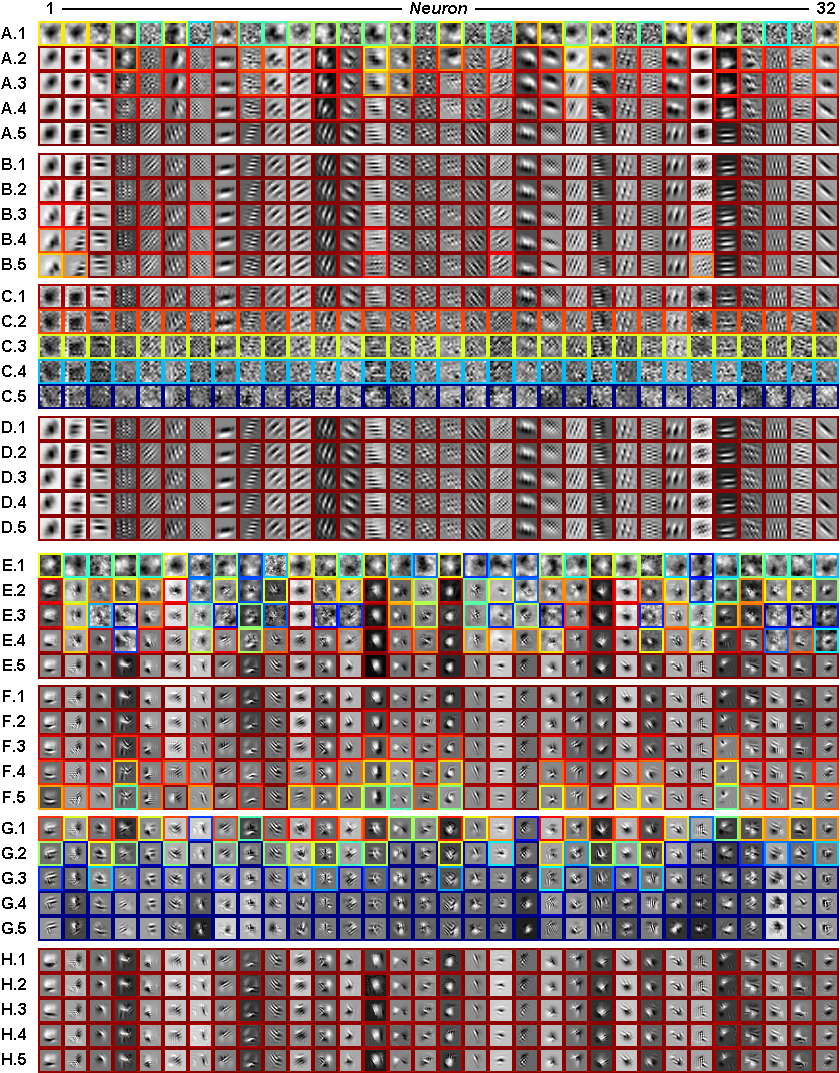
\includegraphics[width=0.90\textwidth]{Figs_supp/pic1.pdf} 
\caption{{\bf Visualization of more shallow and deep representations.}
Color of the boarder of an image indicates the fitness of the representation (\ie response of the neuron) driven by the image, with color map following the definition in the main paper.
A and E show the search trajectories of \emph{optimal stimuli} of all 32 neurons from the best performing shallow and best performing deep networks, respectively, where A.1 and E.1 show the initial $1/f$ random stimuli, A.5 and E.5 the resultant optimal stimuli, and A.2--4 and E.2--4 three intermediate steps corresponding to the three largest curvatures in the fitness histories.
B and F show the \emph{invariance paths} of shallow and deep neurons, starting from the corresponding optimal stimuli show in A.5 and E.5, moving from $0.1\pi$ (B.1 and F.1) to $0.5\pi$ (B.5 and F.5) away accordingly.
C and G show the \emph{selectivity paths} of shallow and deep neurons, with definitions following B and F.
D and H show the \emph{invariance subspaces} sampled $0.1\pi$ away from the optimal stimuli, with 5 out of 20 results randomly selected.
} % do visually
\end{figure}

For optimal stimulus searches, in order to further increase the searching speed, the initial stimulus {was} selected from 1000 ${1}/{f^{\alpha}}$ random stimuli with the best fitness, where $\alpha \in \left\lbrace -4,-3,-2,-1,0 \right\rbrace$, without overly sacrificing the nature of random initialization.
From the results, first, the response landscapes of deep neurons are noticeably more complex than those of shallow neurons, as a large fraction of search trajectories for deep neurons actually go down then up before reaching the (local) optima, which also suggests the numerical solver can handle non-convexity reasonably well.

%\clearpage

\subsection{Invariance and Selectivity Path Potential}
More data related to the invariance and selectivity path potentials are presented in the following figure.

\begin{figure}[H]
\centering 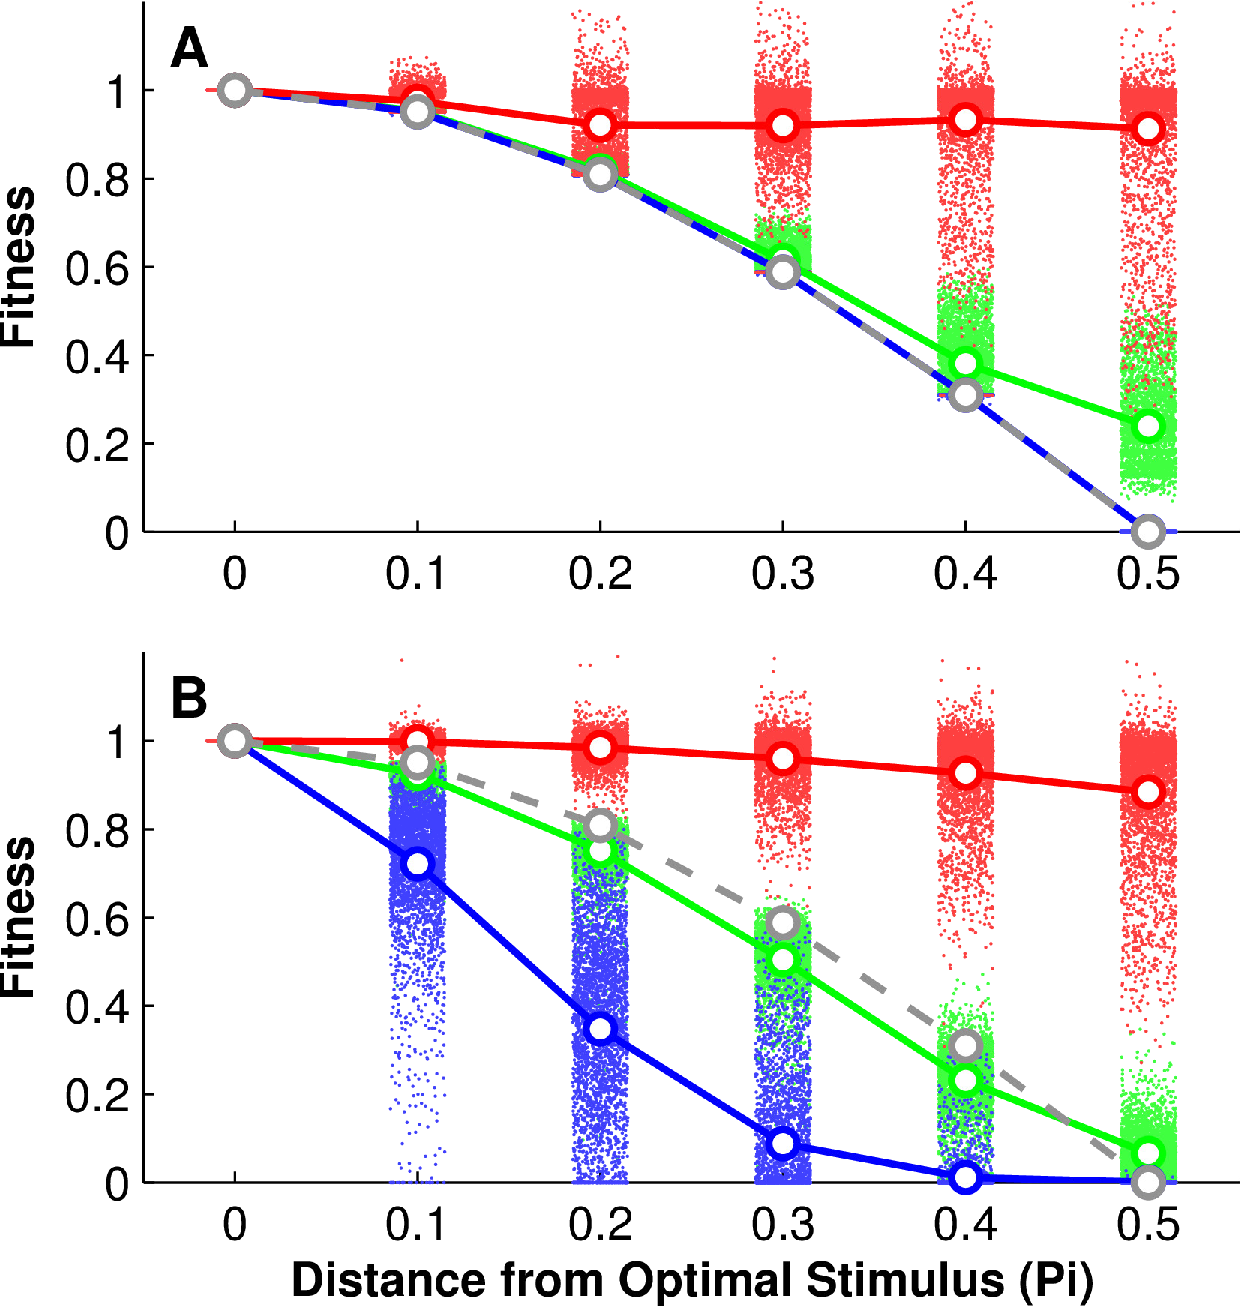
\includegraphics[width=0.60\textwidth]{Figs_supp/e_fig3a_2-nup-crop.pdf} 
\caption{{\bf Fitness-distance analyses of shallow and deep representations with random walk results.} %scalar
In addition to the invariance and selectivity paths, the random perturbation based characterization (\ie random walk results as green dots) of the landscape (\cite{jones1995fitness}, as the original method) was also adopted in our experiments.
A random walk direction can be defined as $f\left(\cos\left(\delta\right)\hat{\bf{x}} + \sin\left(\delta\right)\tilde{\bf{x}}\right)$ where $\tilde{\bf{x}}$ is any random stimulus such that $\left\| \tilde{\bf{x}} \right\| = 1$ and $\left\langle \hat{\bf{x}},\tilde{\bf{x}} \right\rangle = 0$, which can be obtained through random projection of $\mathrm{Null}\left(\hat{\bf{x}}\right)$.
1,000 random walks were executed on each shallow and deep neurons.
The results indicate random walks are not as effective as the numerically optimized results (\ie the invariance and selectivity paths) at characterizing the dynamic range of neurons. 
Nevertheless, comparing the gaps between the random-walk and selectivity curves in A and B also points out that the selectivity of deep neurons is in fact way more ``selective'' (\ie not noise-like) than of shallow neurons.
}
\label{fig:fda}
\end{figure}

\clearpage

\section{Results: Good \vs Bad Representations}

\subsection{Task-related Stimulus Encoding Accuracy}
%Encoding accuracy as a single measure can best explain the deep network's performance. Though bearing strong similarity to the invariance path search in terms of mathematical formulation, encoding accuracy is in fact a radically different and complementary measure, since its numerical optimization is not constrained through distances to the reference stimulus (while distance constraints can induce \emph{a priori} similarities); thus, it can better function as an unconstrained ``global'' characterization of the ``encoding landscape'' and estimate if the (inverted) stimuli that a deep network is invariant to are ``selective'' (\ie visually similar to original stimuli).
More related data are presented in the following 2 figures.

\begin{figure}[H]
\centering 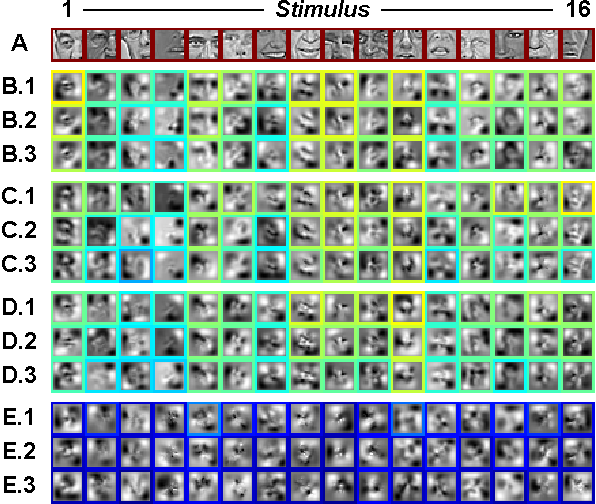
\includegraphics[width=0.55\textwidth]{Figs_supp/pic4.pdf} 
\caption{{\bf More examples of task-related stimulus encoding accuracy.}
Utilizing 16 face images in A as reference stimuli, 3 examples of inverted stimuli from deep networks corresponding to the best, second best, third best and worst average qualities (SSIM) of inverted stimuli are shown in B--E respectively.
Color of the boarder of an image indicates the SSIM between the image and reference stimulus, with color map following the definition in the main paper.
Though the inverted stimuli are in general of lower spatial frequencies, some of the better ones do capture the spatial structures of reference stimuli decently well (\eg stimulus 1, 5, \etc).
} % (reconstructed)
\label{refstim1}
\end{figure}

\begin{figure}[H]
\centering 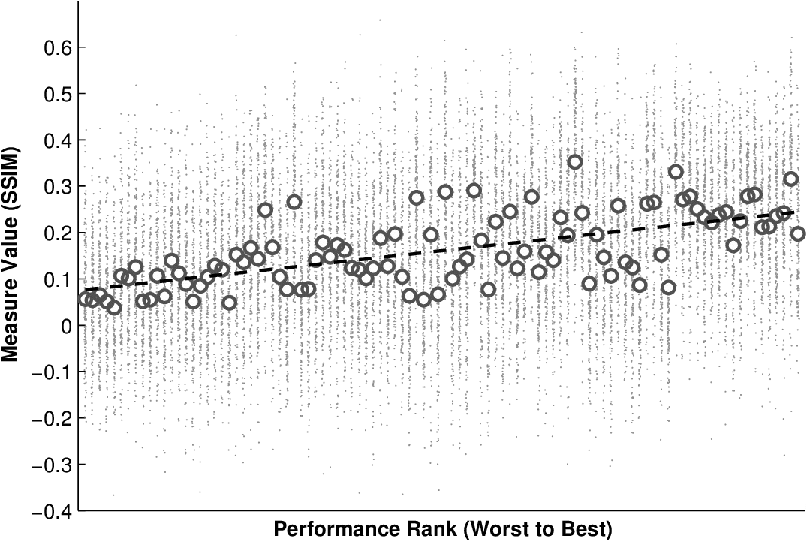
\includegraphics[width=0.60\textwidth]{Figs_supp/e_fig6b-crop.pdf}
\caption{
{\bf Encoding accuracies \vs performances of deep networks.} Each distribution from left to right shows the SSIM scores of the inverted stimuli of vector representations of a deep network against all the 16 reference stimuli (as in Fig.~\ref{refstim1}) in all 10 runs. Means of distributions are plotted as gray circles and the linear regression as dashed black line. %Significance of the slope of all means under permutation test has $p < 0.001$.
}
\end{figure}

\clearpage

\subsection{Invariance and Selectivity \vs Task-related Stimulus Subspace Alignment}
More data related to the subspace alignment measure are presented in the following 2 figures.

\begin{figure}[H]
\centering 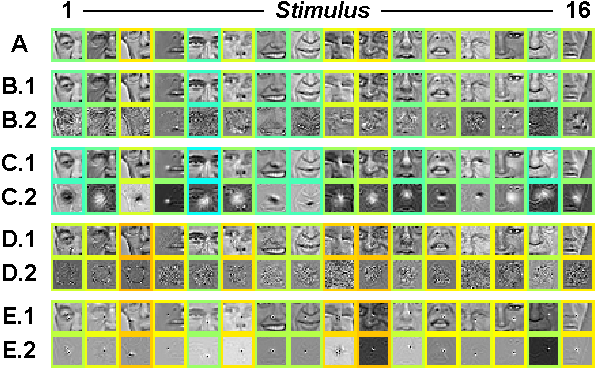
\includegraphics[width=0.55\textwidth]{Figs_supp/pic3.pdf} 
\caption{{\bf More examples of alignments between subspaces of invariance and selectivity paths and task-related stimuli.}
Using 16 face images in A as reference stimuli, the invariance paths at $\delta = 0.1\pi$ corresponding to the best alignments against task-related stimuli (\ie high $L^1$ sparsities of images represented in eigenface coordinates) among all deep networks are shown in B.1, and similarly, best alignments of selectivity paths in C.1, worst alignments of invariance paths in D.1, and worst alignments of selectivity paths in E.1.
Differences between A and B.1--E.1 are shown in B.2--E.2 for clearer visualization.
Color of the boarder of an image indicates the alignment of the image against task-related stimuli, with color map following the definition in the main paper.
While good alignments (B.1 and C.1) appear more natural (like structural deformations, lighting changes, \etc), bad alignments are mostly meaningless noises.
} %of subspaces % which are known to be important factors in visual recognition % accordingly
%Multiple runs of invariance and selectivity path searches are executed to form samples of the subspaces.
\label{refstim2}
\end{figure}

\begin{figure}[H]
\centering 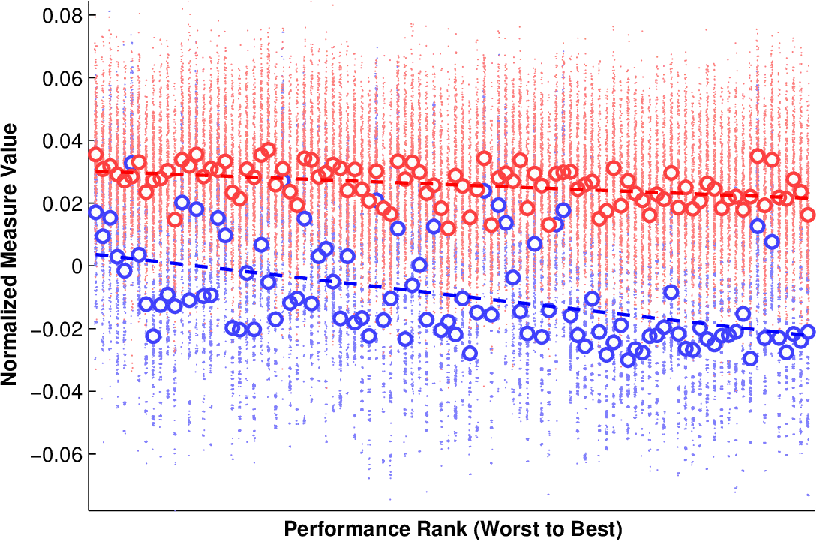
\includegraphics[width=0.60\textwidth]{Figs_supp/e_fig5d-crop.pdf}
\caption{ 
{\bf Invariance and selectivity subspace alignments \vs performances of deep networks.} Each red distribution from left to right shows the invariance subspace alignments against the task-related stimuli in vector representations of a deep network given the 16 reference stimuli (as in Fig.~\ref{refstim2}) in all 20 runs. Alignment scores are normalized by subtracting the corresponding reference stimuli's own alignment scores. Means of distributions are plotted as red circles and the linear regression as dashed red line. Blue distributions for selectivity subspace alignments follow the same definitions.
%Significances of slopes of means under permutation tests both have $p < 0.001$.
}
\end{figure}

\clearpage

\subsection{Optimal \vs Task-related Stimulus Alignment}
More data related to the optimal \vs task-related stimulus alignment measure are presented in the following 2 figures.

\begin{figure}[H]
\centering 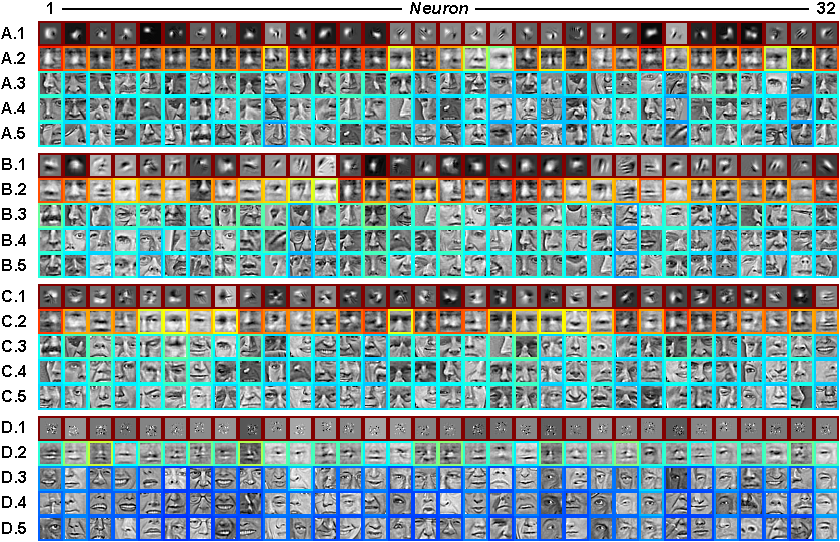
\includegraphics[width=0.90\textwidth]{Figs_supp/pic2.pdf} 
\caption{{\bf More examples of optimal \vs task-related stimulus alignment.}
Results from deep networks of the best 3 average alignment scores (A--C) and the worst average alignment score (D) are visualized.
Within each panel, the first row shows all 32 neurons' optimal stimuli from the network, the third to fifth rows show face images with the top 3 alignment scores (\ie inner-product distances between the images and the corresponding optimal stimuli), and the second row shows the average of images with top 100 alignment scores, out of 10,000 natural images.
Color of the boarder of an image indicates the alignment score of the image, with color map following the definition in the main paper.
}
\end{figure}

\begin{figure}[H]
\centering 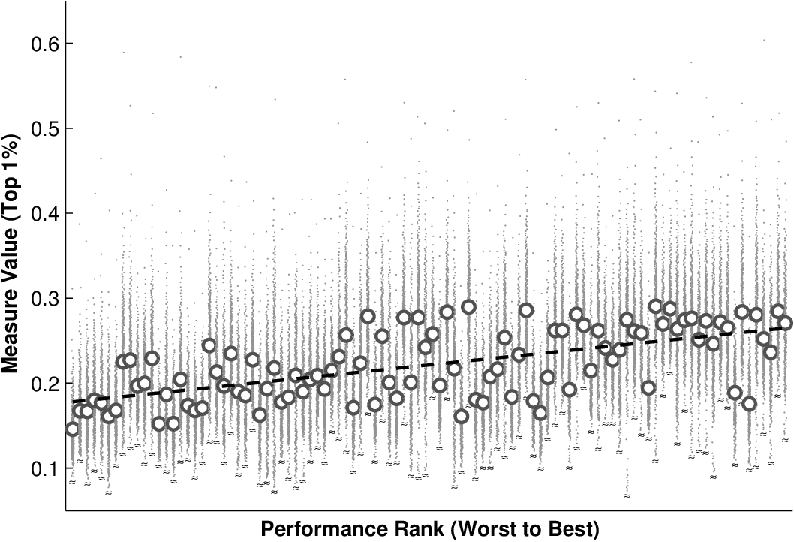
\includegraphics[width=0.60\textwidth]{Figs_supp/e_fig4b-crop.pdf} 
\caption{ 
{\bf Optimal stimulus alignments \vs performances of deep networks.} Each distribution from left to right shows the top 1\% alignment scores of all the 32 top-layer scalar representations of a deep network against the task-related stimuli. Means of distributions are plotted as gray circles and the linear regression as dashed black line.
%Significance of slope of means under permutation test has $p < 0.001$.
}
\end{figure}

\clearpage

\subsection{Invariance and Selectivity Path Potential of Vector Representations}
Since no baseline can be defined for vector representations as for scalar representations , the invariance (and selectivity, similarly) path potential is redefined as path integral on the fitness landscape $\int_{0}^{\frac{\pi}{2}}{\exp\left(-\left\|f\left(\bf{x}^{+}_{\delta}\right)-f\left(\hat{\bf{x}}\right)\right\|\right)}\mathrm{d}\delta \mathbin{/} {\frac{\pi}{2}}$.
More data related to path potential of vector representations are presented in the following figure.

\begin{figure}[H]
\centering 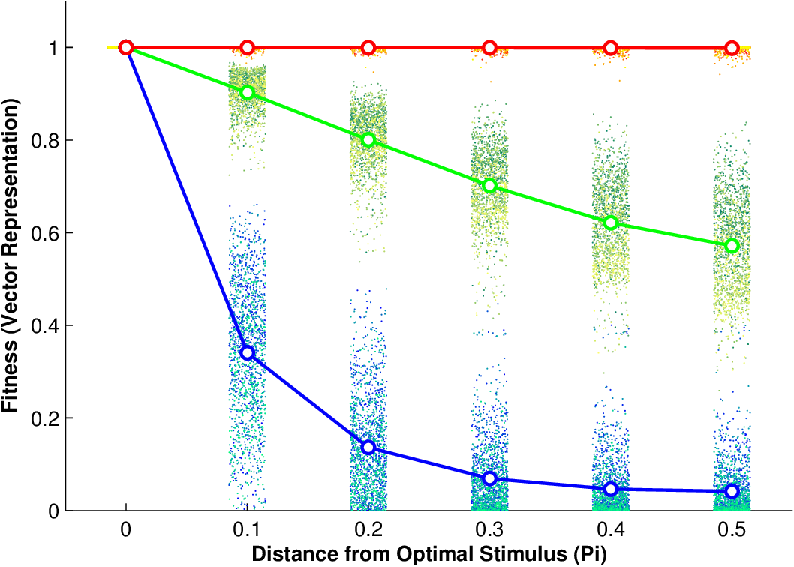
\includegraphics[width=0.60\textwidth]{Figs_supp/e_fig5a-crop.pdf}
\caption{ 
{\bf Fitness-distance analysis of deep vector representations.} Red, blue, and green dots correspond to results of invariance and selectivity path searches, and random walks, starting from all the 16 reference stimuli (as in Fig.~\ref{refstim1}/\ref{refstim2}), where brighter shades of a color are from better performing networks, and darker shades from poorer performing networks. Means of results are plotted as solid lines in corresponding colors. As visualized, correlations between invariance and selectivity path potentials and performance are weak. Random walk results \vs performance, on the other hand, has $\rho = -0.43$ correlation which may arise from the differences in sensitivities to noises, though incorporating it into representation measures does not improve the final multiple correlation.}
\end{figure}

\subsection{Invariance Subspace Capacity of Vector Representations}
More data related to the invariance subspace capacity of vector representations are presented in the following figure.

\begin{figure}[H]
\centering 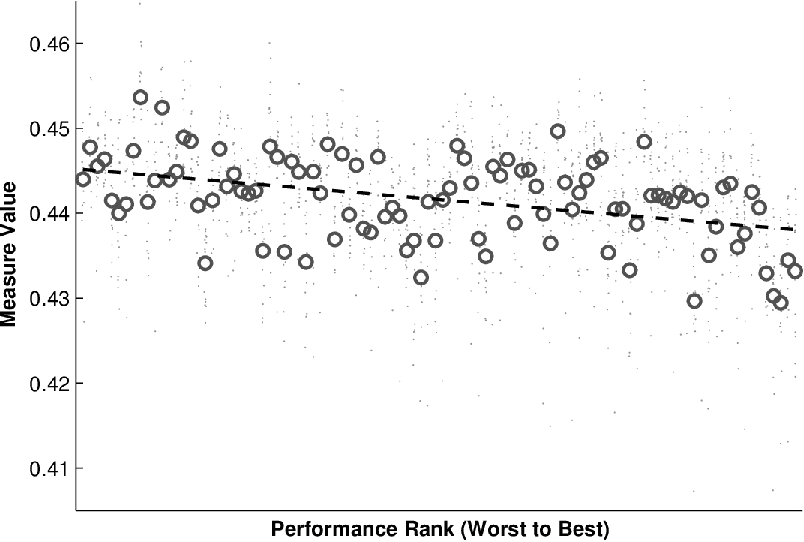
\includegraphics[width=0.60\textwidth]{Figs_supp/e_fig5b-crop.pdf}
\caption{ 
{\bf Invariance subspace capacities \vs performances of deep networks.} Each distribution from left to right shows the invariance subspace capacities of vector representations of a deep network given the 16 reference stimuli (as in Fig.~\ref{refstim1}/\ref{refstim2}). Means of distributions are plotted as gray circles and the linear regression as dashed black line.
%Significance of slope of means under permutation test has $p < 0.001$.
}
\end{figure}

\clearpage

\subsection{Overall Comparison}

More data related to the measures used but not presented in the main paper are presented in the following figure.

\begin{figure}[H]
\centering 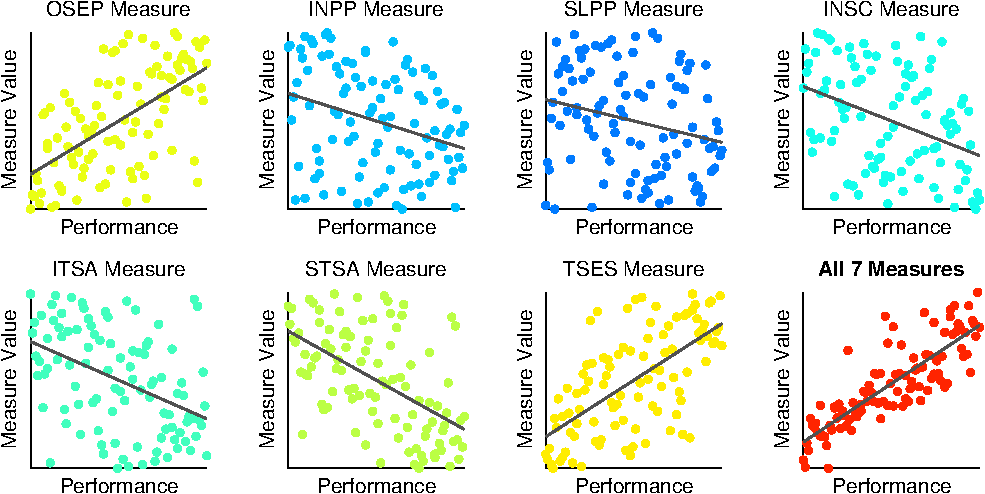
\includegraphics[width=0.65\textwidth, trim=25ex 27ex 0 0, clip]{Figs_supp/e_fig7_scatter.pdf}
\caption{ 
{\bf Invariance and selectivity path potentials (INPP/SLPP), and invariance subspace capacity (INSC) of vector representations \vs performance of networks.} Spearman's rank correlations and their significance levels of INPP, SLPP and INSC are $-0.31^{\ast\ast}$, $-0.24^{\ast}$, $-0.39^{\ast\ast\ast}$, respectively.
Invariance and selectivity path potentials and invariance subspace capacity for deep vector representations, compared to invariance and selectivity subspace alignments, have lower correlations to network's performance (though still significant), possibly due to their nature of being less task-related than subspace alignment measures (INPP, SLPP, and INSC are measures of search results \emph{started} from task-related images, but not \emph{ended} compared against them, unlike ITSA and STSA).
Vector representation's INSC is negatively correlated to network's performance, mainly due to the fact that poorer performing network's invariance paths are usually noisier (as depicted in Fig.~\ref{refstim2}), and thus should be interpreted differently from scalar representation's INSC.
Task-unrelated measures, \ie OSSC, INPP, SLPP, and INSC of scalar representations as used in Sec.~\ref{sec2}, are significantly worse at explaining a network's performance as one would expect.
}
\end{figure}

As a comparison, Pearson's correlations of TSEA, ITSSA, STSSA, OTSA, INPP, SLPP, INSC, and all measures together, are $0.63$, $-0.41$, $-0.48$, $0.61$, $-0.13$, $-0.14$, $-0.43$, and $0.83$, respectively, which are basically consistent with the Spearman's rank correlations.

%(altogether with linear multiple correlation of only $0.59$, and when combined with the other task-unrelated measures, only bring up the correlation marginally from $0.84$ to $0.86$),

\section{Characterizing Face Pair Matching Decisions}

\begin{figure}[H]
\centering 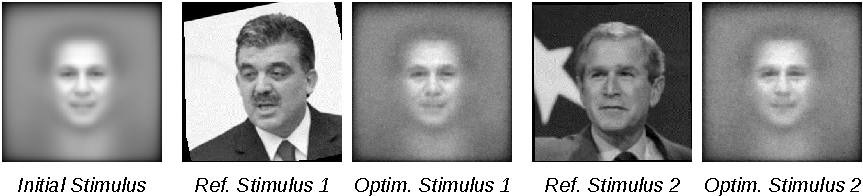
\includegraphics[width=\textwidth]{Figs/whole_face.pdf}
\caption{{\bf Characterizing face pair matching decisions.}
The best-performing decision function $\mathcal{D}$ (\ie the SVM classifier trained based on representations from the best-performing deep network $f_v$) {was} presented with the out-of-training-set reference stimuli, and the optimal stimulus searches, \ie $\arg\max_{\bf{X}}\mathcal{D}(| f_v\left({\bf{X}}\right) - f_v(\tilde{\bf{X}}) |^\frac{1}{2})$, initialized with the LFW-a average face {were} performed.
The resultant optimal stimuli for the ``match'' decisions, though far from photorealism, actually still well capture certain facial features, especially around the eye regions.
}
\label{fig:wface}
\end{figure}

Previous investigations have sought to visualize the optimal stimulus for the decision output of fully trained network \cite{zeiler2014visualizing, simonyan2013deep}, and the methods presented here can also be applied to the final classifier layer in our face matching network.  Fig.~\ref{fig:wface} shows examples of such a procedure, wherein an optimal ``matching'' stimulus was generated starting from an average face. The emergence of distinctive facial features in the optimized image could provide useful information about the features that the network uses to represent matches.

Unlike inverting vector representations, inverting the decision (\ie a single top-layer neuron) back into the entire image $\bf{X}$ is significantly harder, and using the average face (which does not ``match'' any of the reference stimuli) significantly helps with the speed and quality of convergence without biasing the results.
Both resultant optimal stimuli here surprisingly lead to very high matching scores, given that they are merely subtlety different from the average face.
Worth to note, the decision function {was} only trained on 6,000 face pairs.

%and visually carry similarities 
%Why blurry? not inv. rep. it thinks it's close enough. considering the fact that it is only trained on 6,000 face pairs.



{\small
\bibliographystyle{ieee}
\bibliography{ref_supp}
}

\end{document}
